\documentclass[]{article}
\usepackage[T1]{fontenc}
\usepackage{lmodern}
\usepackage{amssymb,amsmath}
\usepackage{ifxetex,ifluatex}
\usepackage{fixltx2e} % provides \textsubscript
% use upquote if available, for straight quotes in verbatim environments
\IfFileExists{upquote.sty}{\usepackage{upquote}}{}
\ifnum 0\ifxetex 1\fi\ifluatex 1\fi=0 % if pdftex
  \usepackage[utf8]{inputenc}
\else % if luatex or xelatex
  \ifxetex
    \usepackage{mathspec}
    \usepackage{xltxtra,xunicode}
  \else
    \usepackage{fontspec}
  \fi
  \defaultfontfeatures{Mapping=tex-text,Scale=MatchLowercase}
  \newcommand{\euro}{€}
\fi
% use microtype if available
\IfFileExists{microtype.sty}{\usepackage{microtype}}{}
\usepackage[margin=1in]{geometry}
\usepackage{color}
\usepackage{fancyvrb}
\newcommand{\VerbBar}{|}
\newcommand{\VERB}{\Verb[commandchars=\\\{\}]}
\DefineVerbatimEnvironment{Highlighting}{Verbatim}{commandchars=\\\{\}}
% Add ',fontsize=\small' for more characters per line
\usepackage{framed}
\definecolor{shadecolor}{RGB}{248,248,248}
\newenvironment{Shaded}{\begin{snugshade}}{\end{snugshade}}
\newcommand{\KeywordTok}[1]{\textcolor[rgb]{0.13,0.29,0.53}{\textbf{{#1}}}}
\newcommand{\DataTypeTok}[1]{\textcolor[rgb]{0.13,0.29,0.53}{{#1}}}
\newcommand{\DecValTok}[1]{\textcolor[rgb]{0.00,0.00,0.81}{{#1}}}
\newcommand{\BaseNTok}[1]{\textcolor[rgb]{0.00,0.00,0.81}{{#1}}}
\newcommand{\FloatTok}[1]{\textcolor[rgb]{0.00,0.00,0.81}{{#1}}}
\newcommand{\CharTok}[1]{\textcolor[rgb]{0.31,0.60,0.02}{{#1}}}
\newcommand{\StringTok}[1]{\textcolor[rgb]{0.31,0.60,0.02}{{#1}}}
\newcommand{\CommentTok}[1]{\textcolor[rgb]{0.56,0.35,0.01}{\textit{{#1}}}}
\newcommand{\OtherTok}[1]{\textcolor[rgb]{0.56,0.35,0.01}{{#1}}}
\newcommand{\AlertTok}[1]{\textcolor[rgb]{0.94,0.16,0.16}{{#1}}}
\newcommand{\FunctionTok}[1]{\textcolor[rgb]{0.00,0.00,0.00}{{#1}}}
\newcommand{\RegionMarkerTok}[1]{{#1}}
\newcommand{\ErrorTok}[1]{\textbf{{#1}}}
\newcommand{\NormalTok}[1]{{#1}}
\usepackage{graphicx}
% Redefine \includegraphics so that, unless explicit options are
% given, the image width will not exceed the width of the page.
% Images get their normal width if they fit onto the page, but
% are scaled down if they would overflow the margins.
\makeatletter
\def\ScaleIfNeeded{%
  \ifdim\Gin@nat@width>\linewidth
    \linewidth
  \else
    \Gin@nat@width
  \fi
}
\makeatother
\let\Oldincludegraphics\includegraphics
{%
 \catcode`\@=11\relax%
 \gdef\includegraphics{\@ifnextchar[{\Oldincludegraphics}{\Oldincludegraphics[width=\ScaleIfNeeded]}}%
}%
\ifxetex
  \usepackage[setpagesize=false, % page size defined by xetex
              unicode=false, % unicode breaks when used with xetex
              xetex]{hyperref}
\else
  \usepackage[unicode=true]{hyperref}
\fi
\hypersetup{breaklinks=true,
            bookmarks=true,
            pdfauthor={Jacques Botes},
            pdftitle={Statistical Inference: Basic inferential data analysis},
            colorlinks=true,
            citecolor=blue,
            urlcolor=blue,
            linkcolor=magenta,
            pdfborder={0 0 0}}
\urlstyle{same}  % don't use monospace font for urls
\setlength{\parindent}{0pt}
\setlength{\parskip}{6pt plus 2pt minus 1pt}
\setlength{\emergencystretch}{3em}  % prevent overfull lines
\setcounter{secnumdepth}{0}

\title{Statistical Inference: Basic inferential data analysis}
\author{Jacques Botes}
\date{September 2014}

\begin{document}

\begin{center}
\huge Statistical Inference: Basic inferential data analysis \\[0.2cm]
\end{center}
\begin{center}
\large \emph{Jacques Botes}\\[0.1cm]
\end{center}
\begin{center}
\large \emph{September 2014} \\
\end{center}
\normalsize


\begin{verbatim}
## Loading required package: ggplot2
## Loading required package: plyr
\end{verbatim}

\subsubsection{Problem Statement}\label{problem-statement}

Load the ToothGrowth data and perform some basic exploratory data
analyses Provide a basic summary of the data. Use confidence intervals
and hypothesis tests to compare tooth growth by supp and dose. (Use the
techniques from class even if there's other approaches worth
considering) State your conclusions and the assumptions needed for your
conclusions.

\subsubsection{About the data}\label{about-the-data}

The response is the length of odontoblasts (teeth) in each of 10 guinea
pigs at each of three dose levels of Vitamin C (0.5, 1, and 2 mg) with
each of two delivery methods (orange juice or ascorbic acid). A data
frame with 60 observations on 3 variables. (taken from
\texttt{?ToothGrowth} in R)

\begin{verbatim}
##       len       supp         dose     
##  Min.   : 4.2   OJ:30   Min.   :0.50  
##  1st Qu.:13.1   VC:30   1st Qu.:0.50  
##  Median :19.2           Median :1.00  
##  Mean   :18.8           Mean   :1.17  
##  3rd Qu.:25.3           3rd Qu.:2.00  
##  Max.   :33.9           Max.   :2.00
\end{verbatim}

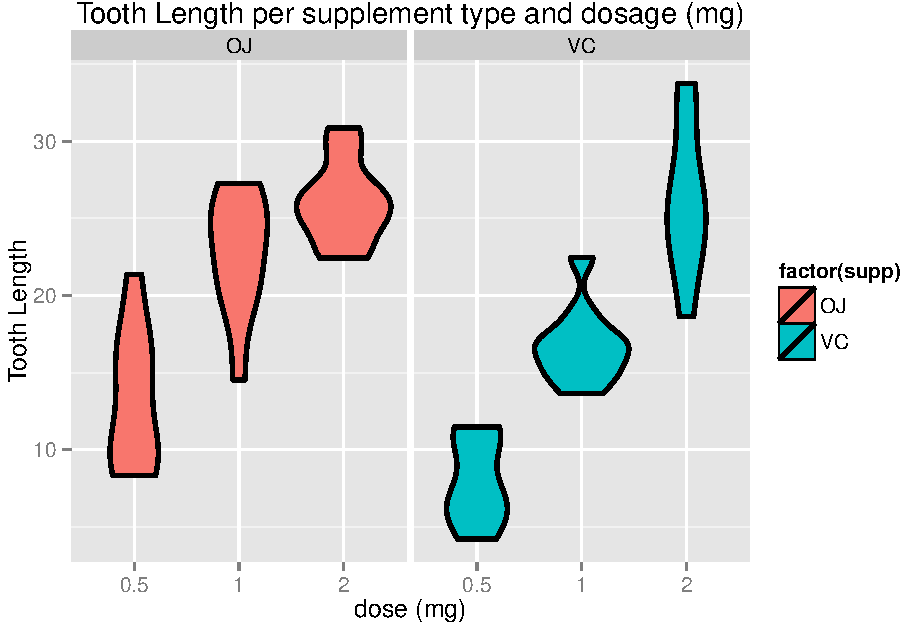
\includegraphics{./Q2_files/figure-latex/exploratory1.pdf}
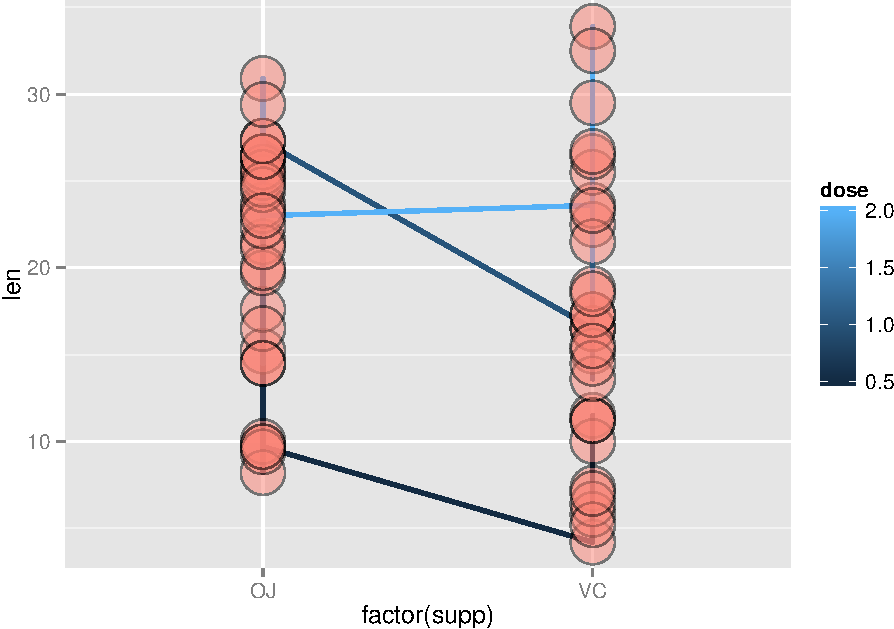
\includegraphics{./Q2_files/figure-latex/exploratory2.pdf}

\subsubsection{Summary of dataset:}\label{summary-of-dataset}

Interpreting the first graph we can see that the Orange Juice (OJ)
supplement at lower doses results in a longer tooth length. With the 2mg
dose the difference in tooth lengh is closely matched and seems to be
working equally well.

\subsubsection{Testing}\label{testing}

\paragraph{Analysis}\label{analysis}

\subparagraph{Test 1}\label{test-1}

Use confidence intervals and hypothesis tests to compare tooth growth by
supp and dose. First test is to test the data only looking at the
supplement and not dosage

\begin{Shaded}
\begin{Highlighting}[]
\KeywordTok{t.test}\NormalTok{(len ~}\StringTok{ }\NormalTok{supp, }\DataTypeTok{paired =} \NormalTok{F,}\DataTypeTok{var.equal=}\NormalTok{F, }\DataTypeTok{data =} \NormalTok{ToothGrowth)}
\end{Highlighting}
\end{Shaded}

\begin{verbatim}
## 
##  Welch Two Sample t-test
## 
## data:  len by supp
## t = 1.915, df = 55.31, p-value = 0.06063
## alternative hypothesis: true difference in means is not equal to 0
## 95 percent confidence interval:
##  -0.171  7.571
## sample estimates:
## mean in group OJ mean in group VC 
##            20.66            16.96
\end{verbatim}

The interval contains the zero value, we cannot reject the null
hypothesis that there isn't a significant difference in tooth length
betwen OJ and VC supplement types.

\subparagraph{Test 2}\label{test-2}

Lets compare specific dosage levels and see if we notice a significant
tooth growth difference. We will test 0.5mg, 1mg and 2mg independently.
We create 3 different subsets of the data and do t level tests for each
one.

\begin{Shaded}
\begin{Highlighting}[]
\NormalTok{tooth.D05 <-}\StringTok{ }\KeywordTok{subset}\NormalTok{(ToothGrowth, dose ==}\StringTok{ }\FloatTok{0.5}\NormalTok{)}
\NormalTok{tooth.D1 <-}\StringTok{ }\KeywordTok{subset}\NormalTok{(ToothGrowth, dose ==}\StringTok{ }\FloatTok{1.0}\NormalTok{)}
\NormalTok{tooth.D2 <-}\StringTok{ }\KeywordTok{subset}\NormalTok{(ToothGrowth, dose ==}\StringTok{ }\FloatTok{2.0}\NormalTok{)}
\end{Highlighting}
\end{Shaded}

\begin{verbatim}
##      [,1]                  [,2]                [,3]              
## [1,] "0.5mg conf interval" "1.71905727146767"  "8.78094272853233"
## [2,] "1.0mg conf interval" "2.80214824916537"  "9.05785175083463"
## [3,] "2.0mg conf interval" "-3.79807046333516" "3.63807046333515"
\end{verbatim}

\begin{verbatim}
##                       mean in group OJ mean in group VC
## [1,] "0.5mg mean est" "13.23"          "7.98"          
## [2,] "1.0mg mean est" "22.7"           "16.77"         
## [3,] "2.0mg mean est" "26.06"          "26.14"
\end{verbatim}

At 2mg the p-value is 0.9639, we cannot reject the null hypothesis that
there isnt a difference in tooth length. The interval also containst 0.
For the other two tests at 0.5 and 1mg we can reject the null
hypothesis. The mean estimate also shows significant differences betwen
OJ and VC at the lower dosage levels.

\subparagraph{Test 3}\label{test-3}

Lets test the differences in dosage levels and see if we notice a
significant tooth growth difference. We will subset the dataset and test
0.5mg with 1mg and 2mg then 1mg with 2mg.

\begin{Shaded}
\begin{Highlighting}[]
\NormalTok{tooth.D05_01 <-}\StringTok{ }\KeywordTok{subset}\NormalTok{(ToothGrowth, dose %in%}\StringTok{ }\KeywordTok{c}\NormalTok{(}\FloatTok{0.5}\NormalTok{,}\FloatTok{1.0}\NormalTok{))}
\NormalTok{tooth.D05_02 <-}\StringTok{ }\KeywordTok{subset}\NormalTok{(ToothGrowth, dose %in%}\StringTok{ }\KeywordTok{c}\NormalTok{(}\FloatTok{0.5}\NormalTok{,}\FloatTok{2.0}\NormalTok{))}
\NormalTok{tooth.D01_02 <-}\StringTok{ }\KeywordTok{subset}\NormalTok{(ToothGrowth, dose %in%}\StringTok{ }\KeywordTok{c}\NormalTok{(}\FloatTok{1.0}\NormalTok{,}\FloatTok{2.0}\NormalTok{))}
\end{Highlighting}
\end{Shaded}

\begin{verbatim}
##      [,1]          [,2]                        [,3]                       
## [1,] "Description" "Confidence Interval Lower" "Confidence Interval Upper"
## [2,] "0.5mg-1mg"   "-11.9837812579016"         "-6.27621874209841"        
## [3,] "0.5mg-2mg"   "-18.1561665388306"         "-12.8338334611694"        
## [4,] "1mg-2mg"     "-8.99648051689202"         "-3.73351948310799"
\end{verbatim}

The p-values for all 3 tests (1.2683 × 10-7, 4.3975 × 10-14, 1.9064 ×
10-5) was very small and therefore we can reject the null hypothesis
that there isnt a significant difference. The higher dosage level in
each test resulted in a longer tooth length.

\subsubsection{Conclusion:}\label{conclusion}

We have conducted three different tests and found the following

\begin{itemize}
\itemsep1pt\parskip0pt\parsep0pt
\item
  When ignoring dose levels: No significant difference in tooth length
  noted
\item
  Taking dosage and supplement into account: Orange Juice (OJ) resulted
  in increased tooth length at lower dosage levels with a insignificant
  difference in length between OJ and VC at the 2mg dosage.
\item
  When ignoring supplement type: Higher dose levels had a significant
  impact on tooth length. There is also a significant impact between the
  different dosages
\end{itemize}

\subsubsection{Assumptions}\label{assumptions}

\begin{itemize}
\itemsep1pt\parskip0pt\parsep0pt
\item
  No other outside factor had a significant impact on the study.
\item
  The variances are different for the seperate populations.
\end{itemize}

The full report including all R code:
\href{}{\url{https://github.com/JacquesBot/StatisticalInference/blob/master/Q2.md}}

\end{document}
